\documentclass[a4paper]{article}

\usepackage{pgfplots}

\pgfplotsset{compat=1.5}
\begin{document}

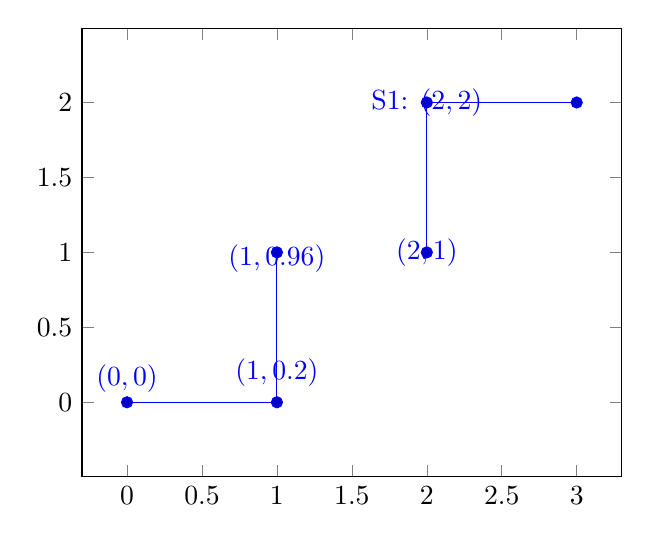
\begin{tikzpicture}
%\tracingmacros=2 \tracingcommands=2
	\begin{axis}[axis equal]
	\addplot coordinates {(0,0) (1,0) (1,1) 
	
		(2,1) (2,2) (3,2)
	}
		node[pos=0,above] {%
			\pgfplotspointplotattime%
			$(
			\pgfmathprintnumber{\pgfkeysvalueof{/data point/x}},
			\pgfmathprintnumber{\pgfkeysvalueof{/data point/y}}
			)$%
		}
		node[pos=0.3] {%
			\pgfplotspointplotattime%
			$(
			\pgfmathprintnumber{\pgfkeysvalueof{/data point/x}},
			\pgfmathprintnumber{\pgfkeysvalueof{/data point/y}}
			)$%
		}
		node[pos=0.49] {%
			\pgfplotspointplotattime%
			$(
			\pgfmathprintnumber{\pgfkeysvalueof{/data point/x}},
			\pgfmathprintnumber{\pgfkeysvalueof{/data point/y}}
			)$%
		}
		node[pos=0.5] {%
			\pgfplotspointplotattime%
			$(
			\pgfmathprintnumber{\pgfkeysvalueof{/data point/x}},
			\pgfmathprintnumber{\pgfkeysvalueof{/data point/y}}
			)$%
		}
		node[pos=0.5,pos segment=1] {%
			\pgfplotspointplotattime%
			S1: 
			$(
			\pgfmathprintnumber{\pgfkeysvalueof{/data point/x}},
			\pgfmathprintnumber{\pgfkeysvalueof{/data point/y}}
			)$%
		}
	;	
	\end{axis}
\end{tikzpicture}
\end{document}

